\documentclass[a4paper,10pt]{article} \usepackage{anysize}
\marginsize{2cm}{2cm}{1cm}{1cm}
%\textwidth 6.0in \textheight = 664pt
\usepackage{xltxtra} 
\usepackage{xunicode} \usepackage{graphicx}
\usepackage{color} \usepackage{xgreek} \usepackage{fancyvrb}
\usepackage{minted}  
\usepackage{enumitem} \usepackage{framed} \usepackage{relsize}
\usepackage{float} \setmainfont[Mapping=TeX-text]{Times New Roman}
\begin{document}

\begin{titlepage}
\begin{center}
\begin{figure}[t] 
     
\includegraphics[scale=0.7]{title/ntua_logo}
\end{figure}
\begin{LARGE}\textbf{ΕΘΝΙΚΟ ΜΕΤΣΟΒΙΟ ΠΟΛΥΤΕΧΝΕΙΟ\\}\end{LARGE}
\vspace{2cm}
\begin{Large}
ΣΧΟΛΗ ΗΜ\&ΜΥ\\
ΤΟΜΕΑΣ ΤΕΧΝΟΛΟΓΙΑΣ ΕΠΙΚΟΙΝΩΝΙΩΝ, ΗΛΕΚΤΡΟΝΙΚΗΣ ΚΑΙ ΣΥΣΤΗΜΑΤΩΝ ΠΛΗΡΟΦΟΡΙΚΗΣ\\
ΕΡΓΑΣΤΗΡΙΟ ΨΗΦΙΑΚΩΝ ΣΥΣΤΗΜΑΤΩΝ\\
1\textsuperscript{η} ΑΣΚΗΣΗ\\
Ακ. έτος 2010-2011\\
\end{Large}
\vspace{5cm}
\Large Τμήμα Γ, Ομάδα 2\textsuperscript{η}\\
\vspace{1cm}
\begin{tabular}{l r}
\Large{Γερακάρης Βασίλης}&
\large{Α.Μ.: 03108137}\\
\Large{Λύρας Γρηγόρης}&
\large{Α.Μ.: 03109687}\\
\end{tabular}\\
\vspace{5cm}

\vfill
\large\today\\
\end{center}
\end{titlepage}



\section*{} \setcounter{section}{1}
\subsection{Σύνδεση με αρχείο αντικειμένων} Ο πηγαίος κώδικας της main.c που
κληθήκαμε να γράψουμε ήταν ο εξής:

\begin{minted}[linenos]{c}
#include "zing.h"
int main(int argc,char ** argv)
{
	zing();
	return 0;
}
\end{minted}

Στη συνέχεια δημιουργήσαμε το makefile για  τη μεταγλώττιση του προγράμματος
με τα εξής περιεχόμενα:

\begin{minted}[linenos]{basemake}

all:	main
main:	main.o
	gcc main.o zing.o -o main -m32 -Wall
main.o:	main.c
	gcc -c -m32 -Wall main.c -o main.o
clean:
	rm main.o main

\end{minted}
Τρέχοντας στο shell την εντολή make έχουμε την παρακάτω έξοδο
\begin{minted}[linenos]{text}
gcc -c main.c -o main.o -Wall -m32
gcc main.o zing.o -o main -Wall -m32
\end{minted}
και τη δημιουργία των αρχείων main.o και του εκτελέσιμου main.\\
Εκτελώντας το main, το πρόγραμμα δίνει την παρακάτω έξοδο:
\begin{minted}[linenos]{text}
oslabb03 ~/code/zing $ ./main
Hello oslabb03!
\end{minted}


\pagebreak
\section*{Απαντήσεις στις θεωρητικές ερωτήσεις}
\subsection{}
Η επικεφαλίδα που χρησιμοποιήσαμε περιέχει τις απαραίτητες  δηλώσεις για τη
διεπαφή των αρχείων κώδικα του προγράμματος μας. 
Η άσκηση αυτή μας παρείχε το object file zing.o , αλλά η συνάρτηση zing( )
δηλώνεται στο zing.h, χωρίς τη χρήση του οποίου δε θα μπορούσαμε να την
καλέσουμε επιτυχώς στη main.

\subsection{}
Απαντήθηκε παραπάνω.


\pagebreak



\subsection*{\textnormal{\underline{Υπολογισμός Αντίστασης R1}}}
Ανάλογα με τους περιορισμούς που είχαμε από τις προδιαγραφές των στοιχείων,
πραγματοποιήσαμε πειραματικές μετρήσεις χρησιμοποιώντας μια κόκκινη φωτοδίοδο
σε σειρά με μια μεταβλητή αντίσταση, ενώ κρατήσαμε σταθερή την τροφοδοσία στα
5V (\textit{Σχήμα 2}). Προσδιορίσαμε έτσι, το άνω και το κάτω όριο της
αντίστασης, λαμβάνοντας ως δεδομένο από το φυλλάδιο προδιαγραφών του 7406 ότι
το μέγιστο ρεύμα που θα επιτρέψουμε να διατρέξει το κύκλωμα είναι 40mA. 
 
\begin{figure}[H] 
\caption{Πειραματική Διάταξη 1.1} 
\centering
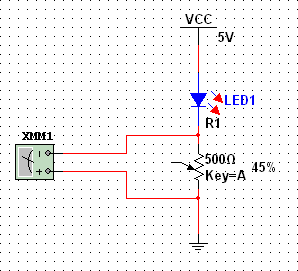
\includegraphics[scale=0.9]{files/peirama1.1.png} 
\end{figure}

\subsubsection*{\textnormal{Υπολογισμός Ελάχιστης Αντίστασης R1}} Η ελάχιστη
αντίσταση προσδιορίζεται από το μέγιστο ρεύμα που επιτρέπουμε να διασχίσει τον
κλάδο 40mA (λόγω της μελλοντικής παρουσίας του 7406). Μεταβάλλοντας κάθε φορά
την αντίσταση, σε διάστημα που επιτρέπει στη δίοδο να φωτοβολεί, μετρήσαμε την
τιμή αυτής καθώς και την τάση στα άκρα της με τελικό σκοπό τον προσδιορισμό
του ρεύματος από το νόμο τον Ohm \begin{math} \mathcal{
I=\frac{V}{R}}\end{math}.  Ενδεικτικά λάβαμε τις παρακάτω μετρήσεις:


\begin{table}[H] 
\caption{Rmin} 
\begin{center} 
\begin{tabular}{|c|c|c|}
\hline
\textbf{V (V)}&\textbf{R (Ω)}&\textbf{I (mA)}\\ 
\hline 3.35&200&16.75\\ 
\hline 3.3&108&30.6\\ 
\hline 3.26&85&38.3\\ 
\hline \end{tabular} 
\end{center}
\end{table} 
Το ρεύμα που αντέχει η δίοδος δεν αποτελεί περιορισμό μιας και
αυτή φωτοβολεί όπως παρατηρήσαμε και όταν διαρρέεται από ρεύμα της τάξης των
70mA το οποίο προφανώς ξεπερνάει τα 40mA. Για την ακρίβεια, μεταβάλλοντας την
αντίσταση μετρήσαμε πως η μέγιστη φωτοβολία της διόδου βρέθηκε για αντίσταση
42Ω πάνω στην οποία μετρήσαμε πτώση τάσης ίση με 3.19V. Επομένως το μέγιστο
ρεύμα που διαρρέει τη δίοδο είναι 
\begin{math}
\frac{3.19V}{42\Omega}={72mA}
\end{math}.  
Η τρίτη μέτρηση δίνει τιμή ρεύματος
ικανοποιητικά κοντά στην επιθυμητή και γνωρίζοντας ότι τα στοιχεία που
χρησιμοποιήσουμε έχουν μεγάλες ανοχές καταλήγουμε χοντρικά ότι 
\begin{math}
R_{min}\simeq80\Omega
\end{math}.  
Υπολογίζουμε θεωρητικά την ελάχιστη τιμή της
αντίστασης λαμβάνοντας την πτώση τάσης στη φωτοδίοδο ίση με 1.8V και από το
Νόμο του Ohm έχουμε: 
\begin{math} R_{min}=\frac{V_{CC} - V_{LED}}{I_{max}} = \frac{5V-1.8V}{40mA} =80\Omega\end{math}
\pagebreak
\subsubsection*{\textnormal{Υπολογισμός Μέγιστης Αντίστασης R1}} Η μέγιστη
αντίσταση αντίστοιχα προσδιορίζεται από το ελάχιστο ρεύμα που επιτρέπει στο
LED να φωτοβολεί ικανοποιητικά.  Όταν, σύμφωνα με τα υποκειμενικά μας κριτήρια,
είχαμε ικανοποιητική ακτινοβολία οι τιμές μου μετρήσαμε με το πολύμετρο
ανέρχονταν σε:


\begin{table}[H] \caption{Rmax} 
\begin{center} 
\begin{tabular}{|c|c|c|} 
\hline
\textbf{V (V)}&\textbf{R (Ω)}&\textbf{I (mA)}\\ 
\hline 3.38&304&11.1\\ 
\hline
\end{tabular} 
\end{center} 
\end{table}

Τα 11.1mA έχουν μικρή απόκλιση από τα 10mA που προσδιορίζονται  ως ελάχιστο
ρεύμα από το datasheet της φωτοδιόδου. Συνεπώς, μπορούμε να θεωρήσουμε ως
\begin{math} R_{max}\simeq300\Omega\end{math}.


Συμπερασματικά, έχουμε ότι:\[ (80\leq R1\leq 300)\Omega \]

Από θεωρητική προσέγγιση, όμοια με προηγουμένως έχουμε ότι \begin{math}
R_{max}=\frac{V_{CC} - V_{LED}}{I_{min}} = \frac{5V-1.8V}{10mA}
=320\Omega\end{math}


Οι αντιστάσεις που προμηθευτήκαμε είναι \begin{math} 220 \Omega \in
[80,300]\Omega \end{math} και συνεπώς κατάλληλες για τη διάταξή μας.


\subsection{Ενδείκτης 7 τμημάτων (7-segment display)} Στο δεύτερο τμήμα της
άσκησης υλοποιούμε τη μετάφραση ενός ψηφίου του κώδικα BCD \textit{(Πίνακας
3)} σε έναν ενδείκτη φωτοδιόδων 7 τμημάτων. Το κύκλωμα αποτελείται από έναν
αποκωδικοποιητή (\textit{SN74LS47N}) και τον ενδείκτη  κοινής ανόδου
(\textit{TOS-5165}). Όπως γνωρίζουμε ο BCD κώδικας χρησιμοποιεί 4 bits με βάρη
8,4,2 και 1 -που αντιστοιχούν στην τιμή της δύναμης του δύο του κάθε bit- για
να παραστήσει τους αριθμούς 0-9. Συνεπώς έχουμε 6 αχρησιμοποίητους συνδυασμούς
των 4 bits. Ο χρησιμοποιούμενος αποκωδικοποιητής έχει καθορισμένη λειτουργία
γι' αυτούς τους μη- επιτρεπτούς αριθμούς BCD και παράγει ειδικές ενδείξεις.
Συνεπώς ουσιαστικά μπορούμε να θεωρήσουμε τον αποκωδικοποιητή σαν 4-16. Όλοι
οι δυνατοί συνδυασμοί όπως κι αυτοί εμφανίστηκαν στον ενδείκτη μας φαίνονται
παρακάτω \textit{(Σχήμα 3)}.

\begin{table}[H] 
\caption{BCD CODE} 
\begin{center} 
\begin{tabular}{|c|c||c|c|}
\hline 0&0000&8&1000\\ 
\hline 1&0001&9&1001\\ 
\hline 2&0010&10&1010\\ 
\hline 3&0011&11&1011\\ 
\hline 4&0100&12&1100\\ 
\hline 5&0101&13&1101\\ 
\hline 6&0110&14&1110\\ 
\hline 7&0111&15&1111\\ 
\hline 
\end{tabular} 
\end{center}
\end{table}

\begin{figure}[h] 
\caption{Απεικόνιση στον ενδείκτη 7 τμημάτων} 
\centering
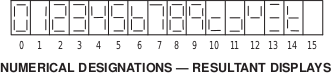
\includegraphics[scale=0.9]{files/7-segment_display.png} 
\end{figure}

\pagebreak
\subsection*{\textnormal{\underline{Κυκλωματική Ανάλυση}}} Το \textit{(Σχήμα
4)} δείχνει τις απαραίτητες συνδέσεις μεταξύ του αποκωδικοποιητή και του
ενδείκτη. Το ΟΚ έχεις τέσσερις εισόδους από τις οποίες η είσοδος D θεωρείται ως
MSB και η είσοδος Α ως το LSB, έτσι τα bits D,C,B και A του ψηφίου BCD
οδηγούνται στις εισόδους 6,2,1 και 7 αντίστοιχα. Εσωτερικά το 7447, μετατρέπει
τις εισόδους σε κώδικα επτά ψηφίων, στις εξόδους 15-19 (\textit{a-g}) , οι
οποίες συνδέονται στη συνέχεια με τα συνονόματα leds  ώστε να σχηματιστεί εκεί
το αποτέλεσμα σε δεκαδική μορφή. Σημειώνεται πως τα pins 9 και 10 του ενδείκτη
αντιστοιχούν στα τμήματα f και g.  Οι ακροδέκτες 3,4,5
(\textit{LT,BI/RBO,RBI}) διατηρούνται στο λογικό επίπεδο H. Για να το
επιτύχουμε αυτό επιλέξαμε να τις συνδέσουμε με την τροφοδοσία αντί να
παραμείνουν στον αέρα καθότι είναι ασφαλέστερη οδός.

\begin{figure}[H] 
\caption{Ενδείκτης 7 τμημάτων} 
\centering
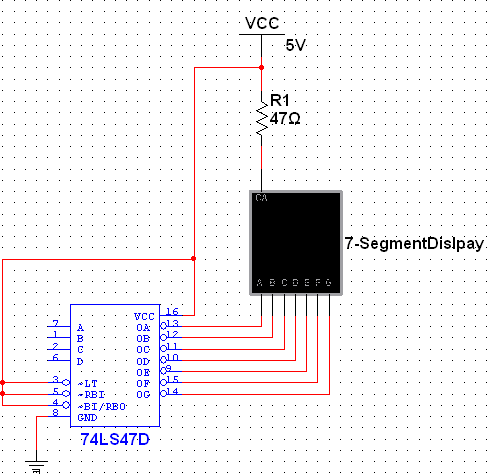
\includegraphics[scale=0.7]{files/7-segment.png} 
\end{figure}

Η είσοδος στον ακροδέκτη 3 ή 8 του ενδείκτη είναι η κοινή άνοδος (\textit{CA})
όλων των LΕD και γειώνεται εσωτερικά από τον 7447. Είναι απαραίτητη η σύνδεση
μια αντίστασης R2 ανάμεσα στον ενδείκτη και την τροφοδοσία, ώστε να παραχθεί
το κατάλληλο ρεύμα στα επιθυμητά LED.

\subsection*{\textnormal{\underline{Υπολογισμός Αντίστασης R2}}}

\subsubsection*{\textnormal{Υπολογισμός Ελάχιστης Αντίστασης R2}} Η ελάχιστη
αντίσταση περιορίζεται από το μέγιστο ρεύμα που μπορεί να δεχθεί το
ολοκληρωμένο.  Το ρεύμα βύθισης του καθένα τρανζίστορ του ΟΚ είναι σύμφωνα με
το datasheet 24mA. Η ελάχιστη απαίτηση από το κύκλωμα εμφανίζεται για το
δεκαδικό ψηφίο 1, όπου χρησιμοποιεί μόνο δύο από τις επτά καταβόθρες. Σε αυτήν
την περίπτωση η R2 διαρρέεται από ρεύμα \begin{math} 2 \ast 24mA = 48mA
\end{math}. Από το Νόμο του Ohm έχουμε: \begin{math} R_{min}=\frac{V_{CC} -
V_{LED}}{I_{max}} = \frac{5V-2.7V}{48mA} \simeq47\Omega\end{math}.


\subsubsection*{\textnormal{Υπολογισμός Μέγιστης Αντίστασης R2}} Σύμφωνα με
τον κατασκευαστή αλλά και τη διευκρίνηση που μας δόθηκε θεωρούμε ότι οι
φωτοδίοδοι λειτουργούν χωρίς καταπόνηση στα 2.7V με ρεύμα 5mA για κανονική
φωτεινότητα. Έτσι η R2 θα διαρρέεται από ρεύμα \begin{math} 7 \ast 5mA = 35mA
\end{math} (έχουμε επτά διόδους). Από το Νόμο του Ohm έχουμε: \begin{math}
R_{min}=\frac{V_{CC} - V_{LED}}{I_{max}} = \frac{5V-2.7V}{35mA}
\simeq66\Omega\end{math}. Η ισχύς που καταναλώνεται ανέρχεται σε \begin{math}
66Ω \ast (35mA)^2 \simeq 80.85mW \end{math}, σαφώς ανεκτή από μια εμπορική
αντίσταση που αντέχει ισχύ μέχρι 250mW.

Συμπερασματικά, έχουμε ότι:\[ (47\leq R2\leq 66)\Omega \].

Η αντίσταση που προμηθευτήκαμε είναι 47Ω, ακριβώς
όπως υποδεικνύεται και από το υποκέφαλαιο 11.5 του Μ.Μano και προσεγγίζει το
κάτω όριο της θεωρητικής μας ανάλυσης εξασφαλίζοντας άριστη λειτουργία. 

\subsubsection*{\textnormal{Πειραματικές Μετρήσεις}} Μετρήσαμε με πολύμετρο
την αντίσταση \begin{math} R2 = 46.6\Omega \end{math}.

Για το δεκαδικό ψηφίο 1 είχαμε τάση \begin{math} V_{R2} = 2.8V \end{math}
οπότε η ελάχιστη απαίτηση από το ρεύμα προσδιορίζεται ως: \[ \bf{Ι_{min}=60mA}
\]

Για το δεκαδικό ψηφίο 8 είχαμε τάση \begin{math} V_{R2} = 3.03V \end{math}
οπότε η μέγιστη απαίτηση από το ρεύμα προσδιορίζεται ως: \[ \bf{Ι_{max}=65mA}
\]

Οι τιμές αυτές κρίνονται ικανοποιητικές για την λειτουργία του κυκλώματος.

\subsection{Διακόπτες Παροχής Λογικών Επιπέδων Τάσεων L,H} Σκοπός του τρίτου
και τελευταίου μέρους της άσκησης είναι η δημιουργία ενός εύχρηστου και
μόνιμου κυκλώματος που θα χρησιμεύει σαν είσοδος δοκιμής για τα επερχόμενα
κυκλώματα. Η υλοποίηση πραγματοποιήθηκε μέσω κυκλώματος που αποτελείται από
έξι μεταγωγικούς διακόπτες κι ένα ΟΚ (\textit{SN74LS04N}) έξι αντιστροφέων.

\begin{figure}[H] \caption{Μεταγωγικοί Διακόπτες} \centering
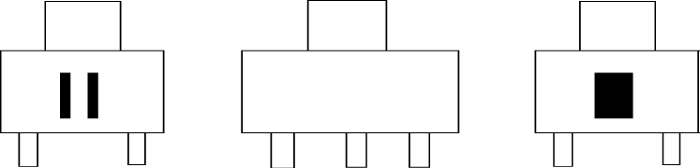
\includegraphics[scale=5.7]{files/diakoptes.png} \end{figure}

Οι διακόπτες που χρησιμοποιούμε για αυτό το μέρος είναι μεταγωγικοί δύο
καταστάσεων και επιτρέπουν την παροχή λογικών επιπέδων  τάσης L και H. Μετά
από δοκιμές με το πολύμετρο καταλήξαμε στα εξής συμπεράσματα: οι έξι
ακροδέκτες χωρίζονται σε δύο ομάδες των τριών, λειτουργικά ανεξάρτητες μεταξύ
τους. Ο κοινός ακροδέκτης κάθε ομάδας είναι ο μεσαίος. Στις δύο από τις
τέσσερις πλευρές υπάρχει μια σήμανση για την εσωτερική λειτουργία του διακόπτη
με την παρουσία μιας ή δύο γραμμών \textit{(Σχήμα 5)}. Από κάθε διακόπτη
χρησιμοποιούμε μόνο τη μία από τις δύο αντιπλευρικές ομάδες έτσι ώστε όταν ο
διακόπτης δεν είναι πατημένος να μας δίνει στον κοινό ακροδέκτη στάθμη H ενώ
όταν πιέσουμε τον διακόπτη, στον κοινό ακροδέκτη να έχουμε στάθμη L.


Οι διακόπτες συνδέονται σε τροφοδοτικό τάσης 5V και στη συνέχεια οι κοινοί
ακροδέκτες οδηγούνται στον αντιστροφέα 7404. Ο αντιστροφέας αυτός έχει έξοδο
τύπου ΤΟΤΕΜ που του επιτρέπει γρηγορότερη απόκριση σε σχέση με το 7406 και τον
καθιστά καταλληλότερο για κυκλώματα τροφοδοσίας λογικών επιπέδων. Επιπλέον το
7406 έχει την ικανότητα οδήγησης μεγαλύτερων ρευμάτων εξόδου, χαρακτηριστικό
που δε θα απαιτηθεί για το αναφερόμενο κύκλωμα.

\end{document}
